\documentclass[12pt, twoside]{article}
\usepackage[letterpaper, margin=1in, head=30pt, headsep=0.1in]{geometry}
\usepackage[english]{babel}
\usepackage[utf8]{inputenc}
\usepackage{amsmath}
\usepackage{amsfonts}
\usepackage{amssymb}
\usepackage{tikz}
\usetikzlibrary{quotes, angles}

\usepackage{graphicx}
\usepackage{enumitem}
\usepackage{multicol}

%\usepackage{pgfplots}
%\pgfplotsset{width=10cm,compat=1.9}
%\usepgfplotslibrary{statistics}
%\usepackage{pgfplotstable}
%\usepackage{tkz-fct}
%\usepackage{venndiagram}

\usepackage{fancyhdr}
\pagestyle{fancy}
\fancyhf{}
\renewcommand{\headrulewidth}{0pt} % disable the underline of the header
\raggedbottom
\newif\ifmeta
\metatrue %print standards and topics tags

\title{High School Geometry problem sets}
\author{Chris Huson}
\date{March 2021}

%\fancyhead[RE]{\thepage}
%\fancyhead[RO]{\thepage \\ Name: \hspace{3cm}}
%\fancyhead[L]{BECA / Dr. Huson / 10th Grade Geometry\\* 7 June 2019}
%
%\begin{document}
%\subsubsection*{13.7 Homework: Cross sections, distance applications}
%\fancyhead[L]{BECA / Dr. Huson / Geometry 03-Volume+angle-bisectors\\* pset ID: 34}

\begin{document}

\subsubsection*{6.17 Exam: Area, volume, and density situations}
\begin{enumerate}

\item Find the area of rectangle $ABCD$ having length $l=18$ and width $w=6 \frac{1}{4}$. Start with a formula of this form, substituting the given values: \\[0.5cm]
$A = l \times w$
  \begin{flushright}
  \begin{tikzpicture}[scale=1.25]
    \draw [-, thick] (0,0)--(4.5,0)--(4.5,2)--(0,2)--cycle;
    \draw [fill] (0,0) circle [radius=0.05] node[left]{$A$};
    \draw [fill] (4.5,0) circle [radius=0.05] node[right]{$B$};
    \draw [fill] (4.5,2) circle [radius=0.05] node[right]{$C$};
    \draw [fill] (0,2) circle [radius=0.05] node[left]{$D$};
    \node at (5, 1){$6 \frac{1}{4}$};
    \node at (2.25, -0.5){$18$};
    %\node at (2.25, 1){$A = 15$};
  \end{tikzpicture}
  %https://graspablemath.com/canvas?load=_fa182d9d9d78d850
  \end{flushright}

\newpage
\item Find the weight of a volume of water of 23 cubic feet given that the density of water is 62.4 pounds per cubic foot.  \\[0.5cm]
$W=V \times D$
%https://graspablemath.com/canvas?load=_4fe25c69e45fccbd

\newpage
\item The $\triangle ABC$ is shown below with $A(2,1)$, $B(7,1)$, and $C(3,5)$. The length of the base of the triangle is $AB=5$.
  \begin{multicols}{2}
    \begin{enumerate}
      \item Write down the height $h$.
      \item Find the triangle's area, showing the substitution into the area formula.\\[0.25cm]
      $A=\frac{1}{2}bh$ \vspace{2cm}
      \end{enumerate}
      \begin{flushright}
      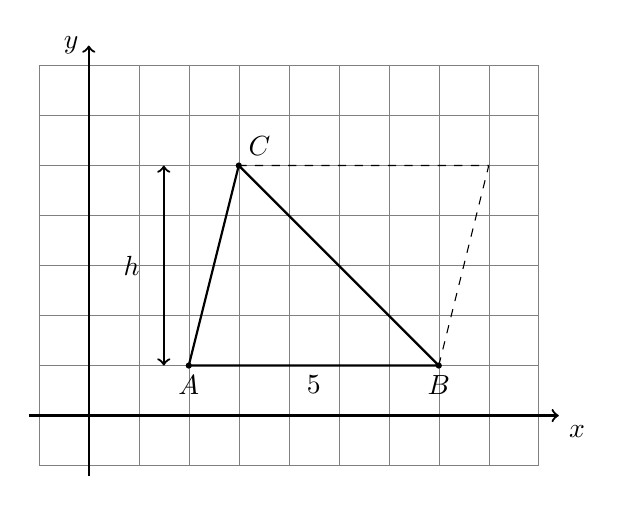
\begin{tikzpicture}[scale=.635]
        \draw [help lines] (-1,-1) grid (9,7);
        \draw [thick, ->] (-1.2,0) -- (9.4,0) node [below right] {$x$};
        \draw [thick, ->] (0,-1.2)--(0,7.4) node [left] {$y$};
        \draw [<->, thick] (1.5,1)--(1.5,5);
        \draw [-, thick] (2,1)--(7,1)--(3,5)--cycle;
        \draw [-, dashed] (7,1)--(8,5)--(3,5);
        \draw [fill] (2,1) circle [radius=0.05] node[below] {$A$};
        \draw [fill] (7,1) circle [radius=0.05] node[below] {$B$};
        \draw [fill] (3,5) circle [radius=0.05] node[above right] {$C$};
        \node at (4.5,1)[below]{$5$};
        \node at (0.5,3)[right]{$h$};
      \end{tikzpicture}
      \end{flushright}
      %https://graspablemath.com/canvas?load=_7190d54aa454877d
  \end{multicols}

\newpage
\item Find the volume of a pyramid having a square base 4 units on each side, $s=4$, and a height of $h=5$. Show the substitution in the volume formula for full credit. \\[0.5cm]
$\displaystyle V = \frac{1}{3} s^2 h$
  \begin{flushright}
    \includegraphics[width=9cm]{6-17-4-pyramid.png}
    %https://graspablemath.com/canvas?load=_84b1e82deef48a75
  \end{flushright}

\newpage
\item The American Eagle \emph{silver} coin is minted by the US Treasury. The one ounce coin has a radius of about $r=20$ millimeters and thickness $h=3$ mm. Given that the density of silver is $D = 0.0105$ grams per cubic millimeter, find the coin's volume and weight. \\[0.25cm]
Show the substitution into both formulas for full credit.\\[0.5cm]
$\displaystyle V = \pi r^2 h$ and $W=VD$
  \begin{flushright}
    \includegraphics[width=6cm]{6-17-5-coin.png}
    %https://graspablemath.com/canvas?load=_845e39ea582acd9e
  \end{flushright}
  
  
\newpage
\item A parallelogram is shown on the $x$-$y$ plane having a base $b=14.5$, unknown height $h$, and area $A=348$. Find the height. 
  \begin{multicols}{2}
    Show the area formula with substituted values for full credit.
      \begin{flushright}
      \begin{tikzpicture}[scale=.8]
        %\draw [help lines] (-1,-1) grid (9,6);
        \draw [thick, ->] (-1.2,0) -- (7.4,0) node [below right] {$x$};
        \draw [thick, ->] (0,-1.2)--(0,6.4) node [left] {$y$};
        \draw [<->, thick] (1.5,1)--(1.5,5);
        \draw [-, thick] (2,1)--(4.75,1)--(5.75,5)--(3,5)--cycle;
        \node at (3.5,1)[below]{$14.5$};
        \node at (1.5,3)[left]{$h$};
        \node at (3.7,3)[]{$A=348$};
      \end{tikzpicture}
      \end{flushright}
  \end{multicols} 

\newpage
\item Find the population density of Brooklyn, New York (Kings County) in people per square mile.\\[0.5cm]
Population estimate July 1, 2019: 2,559,903\\[0.25cm]
Land area in square miles: 69.4
\begin{flushright}
  \includegraphics[width=8cm]{6-15-7-Brooklyn.png}\\
  Source: US Census (census.gov)
  %https://graspablemath.com/canvas?load=_0b517bab59c981c7
\end{flushright}

\newpage
\item The rectangular prism shown has a volume of $V=9911$ cubic centimeters. Its base measures $l=22$ centimeters by $w=13.25$ cm. \\[0.5cm]
Find its height in centimeters. For credit, begin by writing the volume formula with values substituted.
\begin{flushright}
  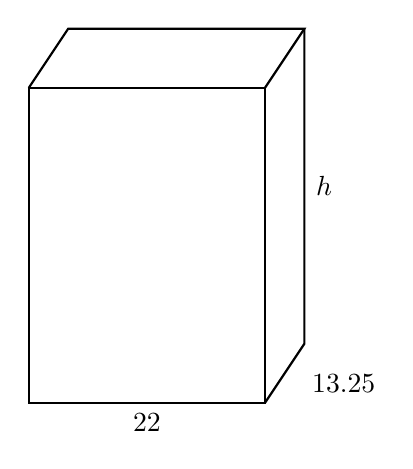
\begin{tikzpicture}[scale=1]
    \draw [-, thick] (0,0)--(3,0)--(3,4)--(0,4)--cycle;
    \draw [-, thick] (0,4)--(0.5,4.75)--(3.5,4.75)--(3,4);
    \draw [-, thick] (3,0)--(3.5,0.75)--(3.5,4.75);
    \node at (3.75, 2.75){$h$};
    \node at (1.5, -0.25){$22$};
    \node at (4, 0.25){$13.25$};
  \end{tikzpicture}
  %https://graspablemath.com/canvas?load=_21d5199065c209a4
\end{flushright}

\newpage
\item Find the radius of a sphere having a volume of 6367.4 cubic inches. Round to \emph{the nearest tenth of an inch}. Show the substitution in the volume formula for full credit. \\[0.5cm]
$\displaystyle V = \frac{4}{3} \pi r^3$
  \begin{flushright}
    \includegraphics[width=8cm]{6-15-9-sphere.png}
    %https://graspablemath.com/canvas?load=_7f185d285c634826
  \end{flushright}

\newpage
\item A building wall must be painted. Each gallon of paint covers 400 square feet and costs \$34.50. If the wall measures 120 feet wide by 45 feet tall, how much will the paint cost? (assume that paint must be purchased in gallon cans)

\end{enumerate}
\end{document}